	% This template is taken from the following 
%       http://www-i6.informatik.rwth-aachen.de/~dreuw/latexbeamerposter.php
\documentclass[final]{beamer}

\newcommand {\cE} {\mathcal{E}}
\newcommand {\cD} {\mathcal{D}}
\newcommand{\E}{\ensuremath{\mathbb{E}} } %
\newcommand {\bxi} {\mbox{\boldmath $\xi$}}%
\newcommand{\bl}{\ensuremath{\mathbf{l}}} %
\newcommand{\bi}{\ensuremath{\mathbf{i}}} %
\newcommand{\bn}{\ensuremath{\mathbf{n}}} %
\newcommand{\bx}{\ensuremath{\mathbf{x}}} %

%\usepackage[absolute,overlay]{textpos}
%
%\setbeamercolor{framesource}{fg=gray}
%\setbeamerfont{framesource}{size=\tiny}
%\newcommand{\source}[1]{\begin{textblock*}{12cm}(1cm,8.6cm)
%    \begin{beamercolorbox}[ht=0.5cm,left]{framesource}
%        \usebeamerfont{framesource}\usebeamercolor[fg]{framesource} Source: {#1}
%    \end{beamercolorbox}
%\end{textblock*}}


\mode<presentation> {
        % you can chose your theme here:
        %  \usetheme{Aachen}
         \usetheme{I6dv}        % the one in use (custom)
		%  \usetheme{I6pd2}
        %  \usetheme{I6pd}
        %            \usetheme{Berlin}
        %               \usetheme[height=10cm]{Rochester}
        %               \usetheme{Madrid}
        %  \usetheme{I6pd2}
        %  \usetheme{I6td}
        %  \usetheme{Oldi6}
}

\graphicspath{{figures/}}

\usepackage{ragged2e, times, wrapfig, graphicx}
\usepackage{amsmath, amssymb, amsfonts, mathrsfs}
\usepackage{graphics,xcolor}
\usepackage[english]{babel}
\usepackage[latin1]{inputenc}
\usepackage[orientation=landscape,size=custom,width=121,height=91,scale=2,debug]{beamerposter}  % e.g. custom size poster

% - - - - - - - - - - - - - - - - - - - - - - - - - - - - - - - - - - - - - - -
        
        \title[Fancy Posters]{Minimum Time Control in SCARA Robot Simulation}
        \author{Sam Tormey, Nick Link, Rick LeVan. Advisor: Matthias Heinkenschloss}
        \institute{Department of Computational and Applied Mathematics, Rice University}
        
        
        
\begin{document} %%%%%%%%%%%%%%%%%%%%%%%%%%%%%%%%%%%%%%%%%%%%%%%%%%%%%%%%%%%%%%
        \begin{frame}{}
        
        \vfill
        %\vspace{-1cm}
		\vspace{0cm}
% =============================================================================
%                                     Column 1
% =============================================================================
{\footnotesize
\begin{columns}[t]
        
\hspace{0.7cm}
\begin{column}{.30\linewidth}
                
\begin{block}{\centering Introduction}
Improving the efficiency of recycling through automation was the inspiration for our project.    \\

%\vspace{0.8cm}

\begin{columns}[T]
\begin{column}{16cm}{}
	\vspace{0.5cm}
	\centering 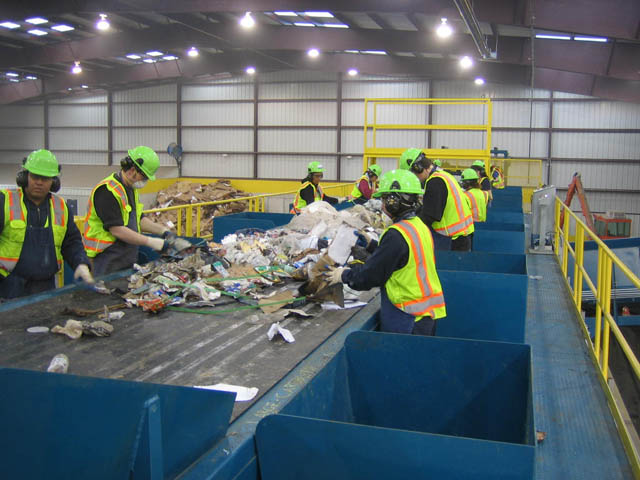
\includegraphics[height=10cm, width = 12cm]{figures/mrf-recycling-system.jpg}\\
\end{column}
\begin{column}{16cm}{}
	\centering 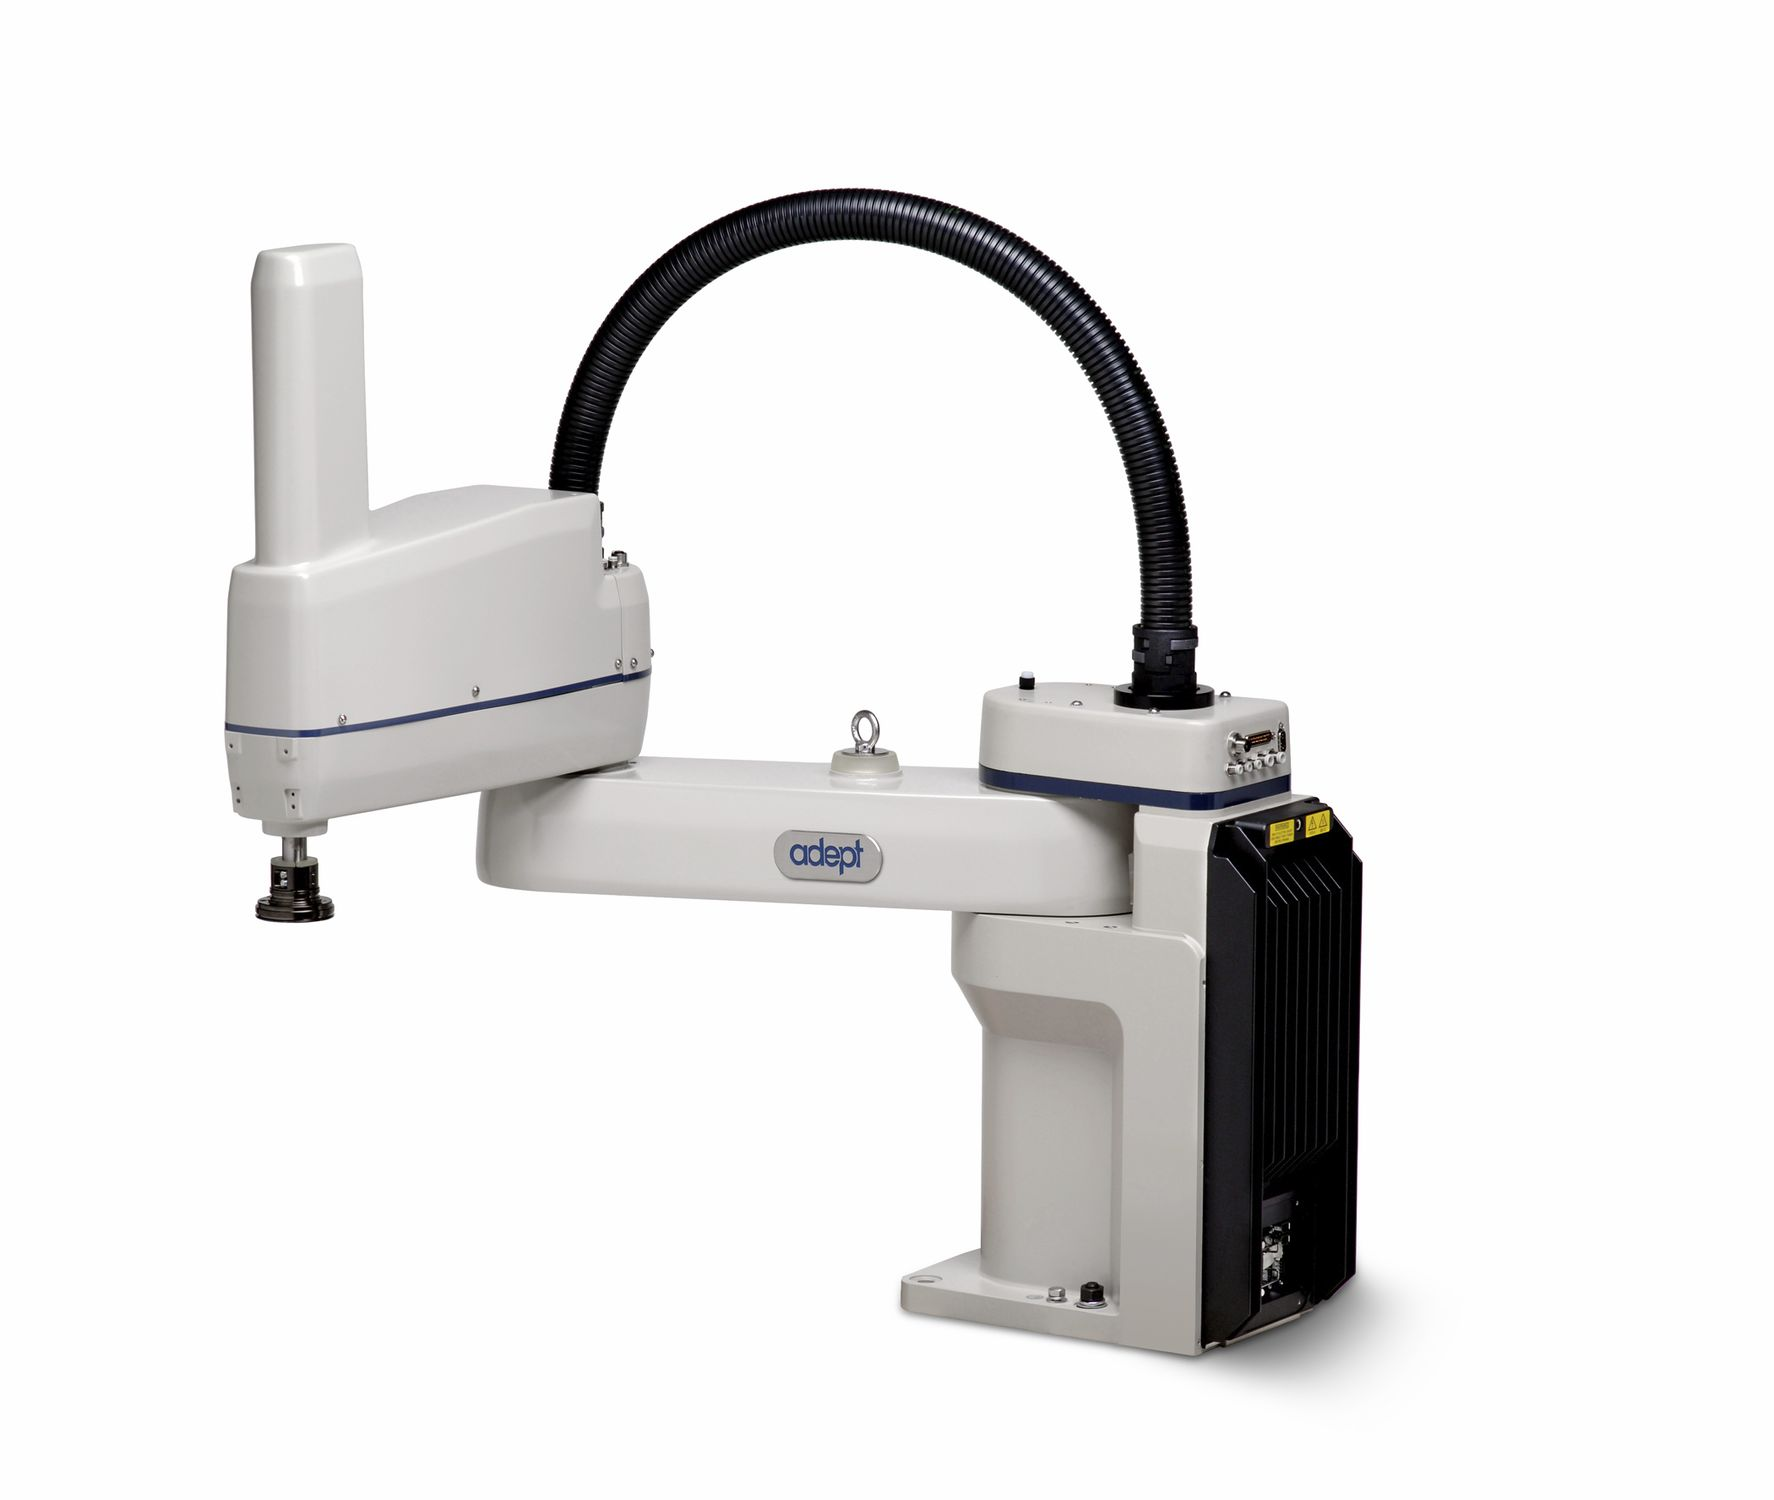
\includegraphics[height=12cm, width = 14cm]{figures/scara.jpg}\\
\end{column}


\end{columns}

\vspace{0.3cm}



We model the removal of objects from a conveyor belt with a MATLAB simulation of a SCARA robot.\\

We solve a constrained optimization problem to find the optimal path between starting and
ending configurations. \\
 
\end{block}
                
%-*-*-*-*-*-*-*-*-*-*-*-*-*-*-*-*-*-*-*-*-*-*-*-*-*-*-*-*-*-*-*-*-*-*-*-*-*-*-*-*-*-*-*-*
                
%\vspace{1cm}

\begin{block}{\centering Double Pendulum Physics} 

We calculate the kinetic energy of our system as

\vspace{-0.5cm}
	
\begin{align*}
	E = \frac{1}{2}\dot\theta_1^2(I_4 + 2I_5\cos\theta_2)
	+ \frac{1}{2}\dot\theta_2^2I_6
	+ \dot\theta_1\dot\theta_2(I_3 + I_5 \cos\theta_2)
\end{align*}

where the $I_j$ terms represent moments of inertia. 

We ignore gravity and thus potential energy. The Euler-Lagrange equation then applies
only to the kinetic energy above:

\begin{columns}[T]
\begin{column}{16cm}{}
	\vspace{0.7cm}
\[ \scalebox{2.3}{$\frac{\partial E}{\partial \theta_j} - \frac{d}{dt}\frac{\partial E}{\partial \dot{\theta_j}} = u$}\]
where $u$ is the vector of torque at the actuators
\end{column}
\begin{column}{16cm}{}
\centering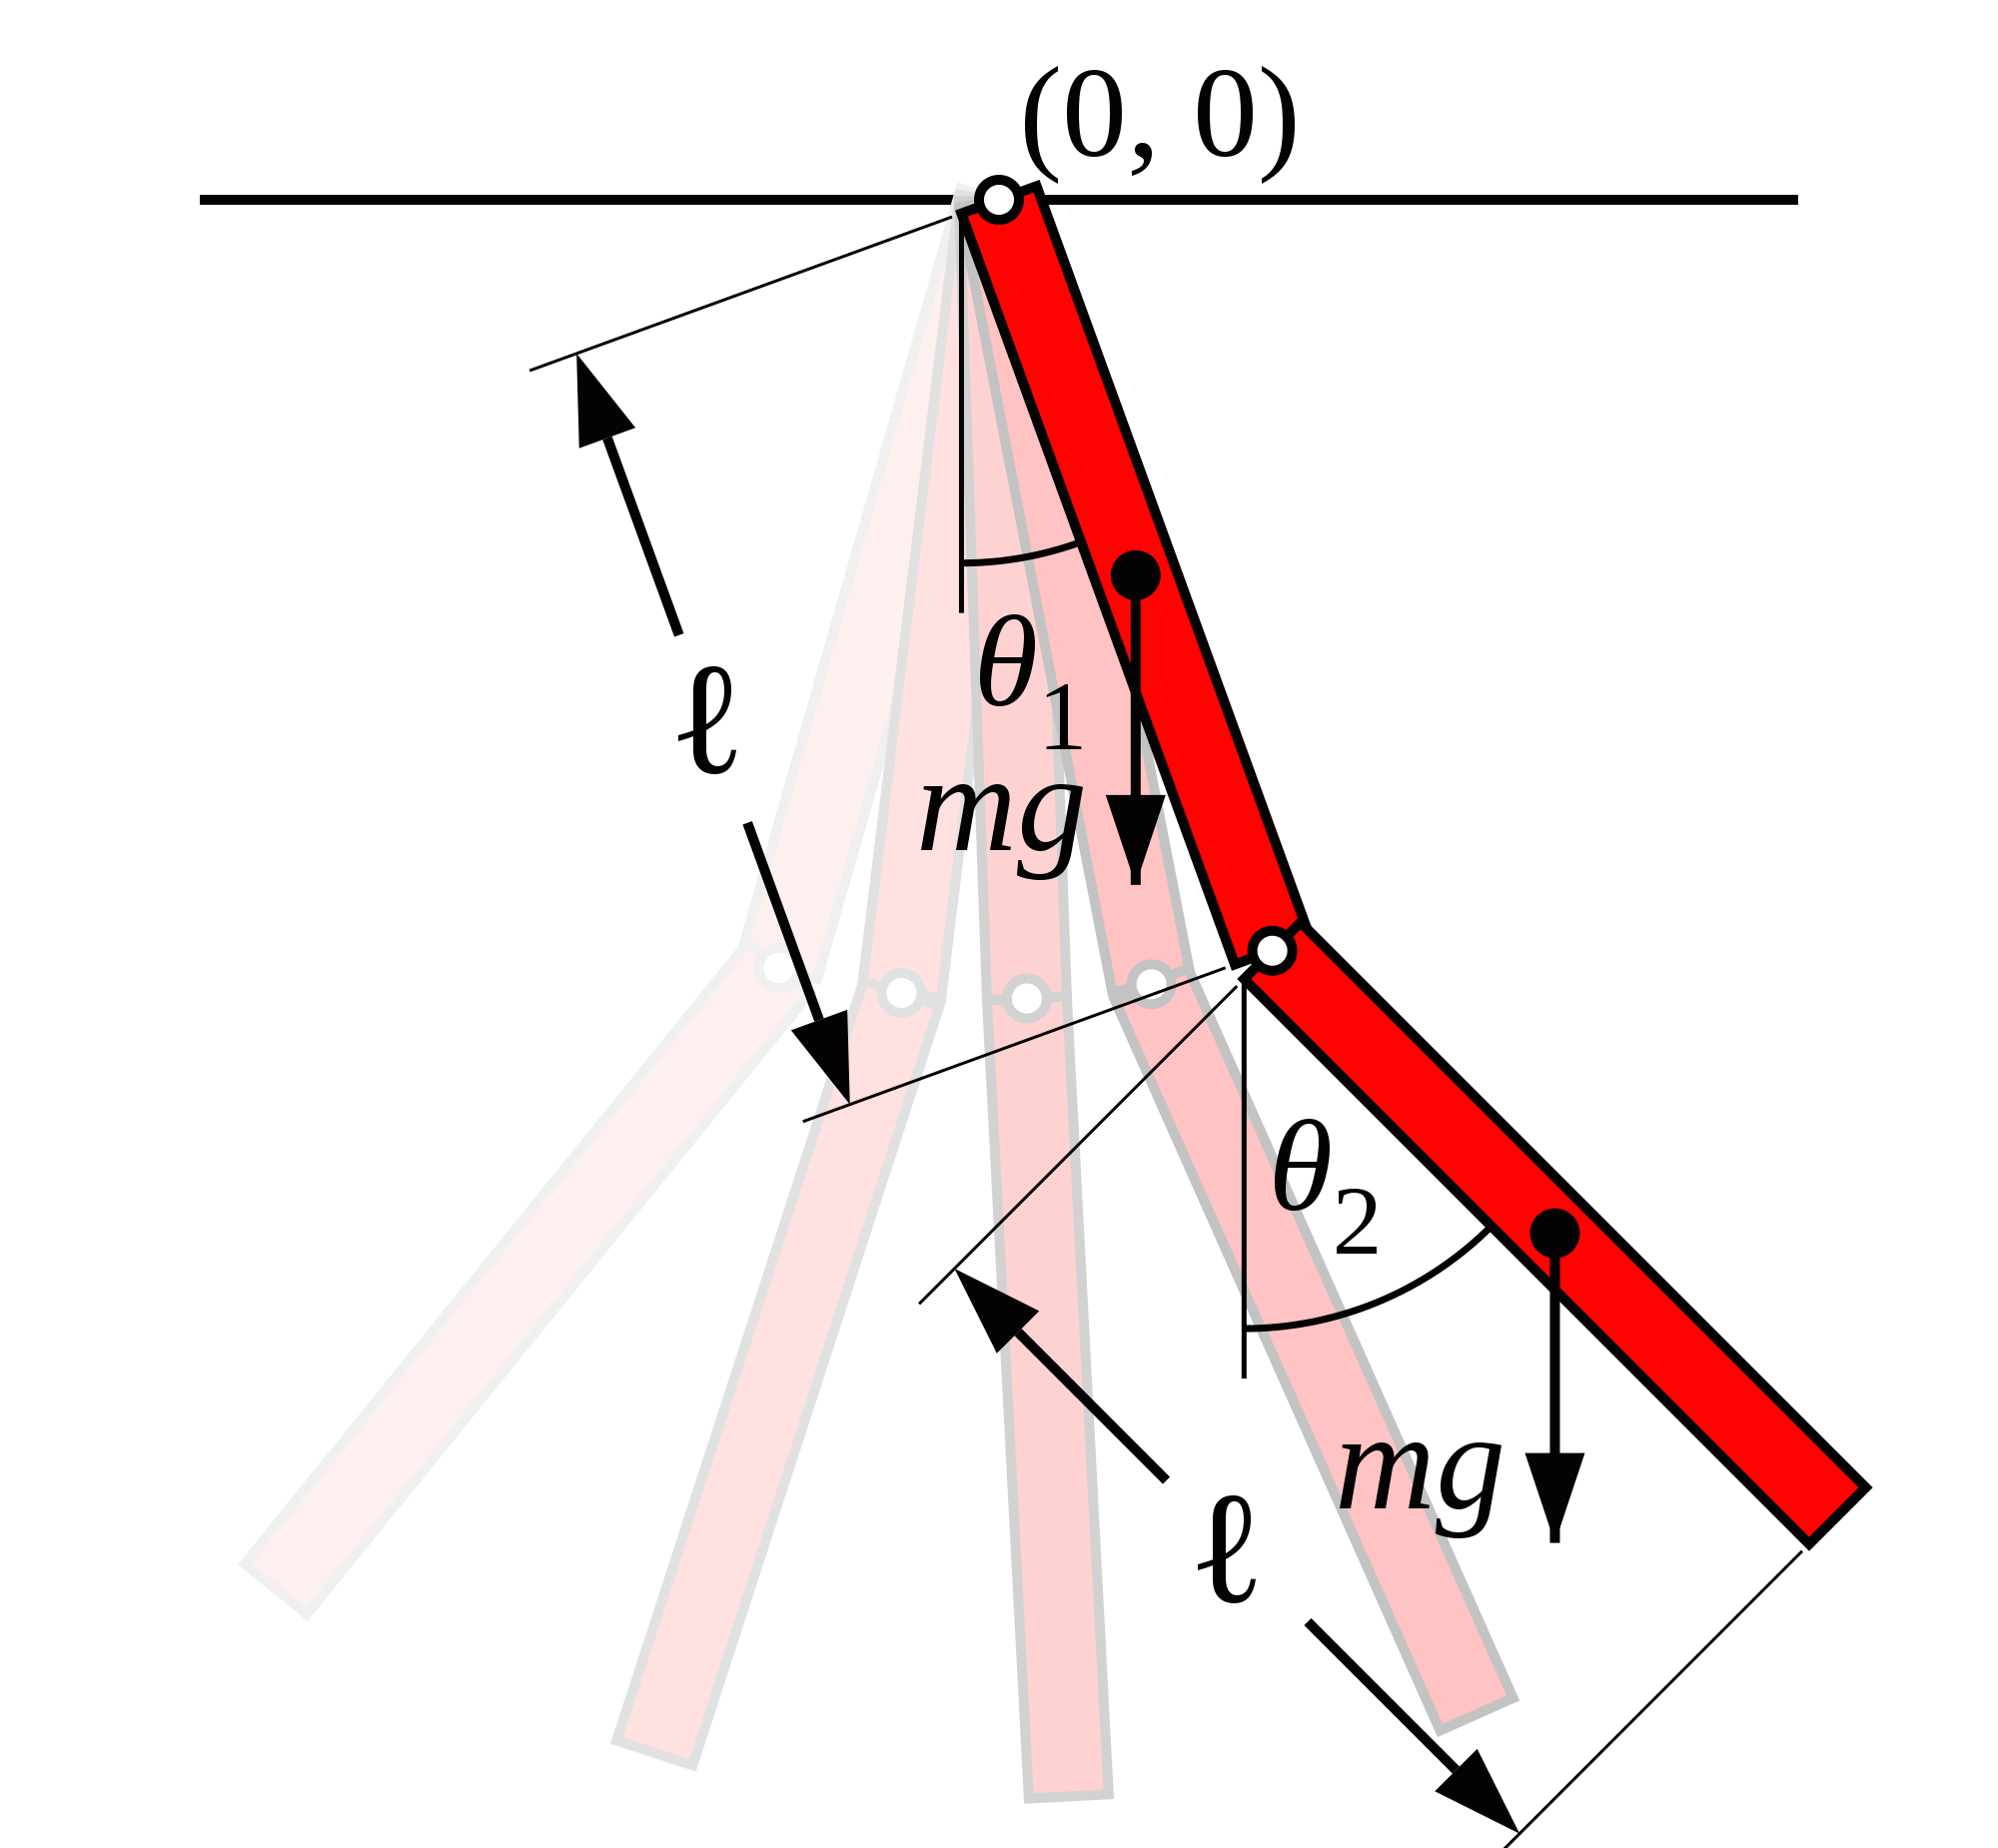
\includegraphics[height=10cm, width = 10cm]{figures/double-pendulum.png}\\
\end{column}

\end{columns}

\end{block}

                
%-*-*-*-*-*-*-*-*-*-*-*-*-*-*-*-*-*-*-*-*-*-*-*-*-*-*-*-*-*-*-*-*-*-*-*-*-*-*-*-*-*-*-*-*
                
%\vspace{1cm}

\begin{block}{\centering The Optimization Problem}


\begin{columns}[T]

\begin{column}{10cm}{}

	\underline{Original Problem}
\begin{align*}
\min  & \: \:T \\
\mbox{s.t. } & \frac{dx(t)}{dt} = f(x(t),u(t)) \\
& x(0) = x_0 \\
& x(T) = x_T \\
& t \in [0, T]
\end{align*}



\end{column}

\begin{column}{12cm}{}

	\underline{Discretized Problem}
\begin{align*}
\min  & \: \:T \\
	\mbox{s.t. } & \frac{x_{j+1}-x_j}{\Delta\tau} = Tf(x_j,u_j) \\
& x_1 = x_0 \\
& x_n = x_T \\
& 1 \leq j \leq n
\end{align*}
\end{column}

\end{columns}


where 
\begin{itemize}
\item $T$ = total time taken by path 
\item $t$ = time 
\item $x(t)$ = state at time $t$ 
\item $u(t)$ = control at time $t$ 
\item $x_0$ = initial state
\item $x_{\scriptsize\mbox{T}}$ = end state
\end{itemize} 

\end{block}


%-*-*-*-*-*-*-*-*-*-*-*-*-*-*-*-*-*-*-*-*-*-*-*-*-*-*-*-*-*-*-*-*-*-*-*-*-*-*-*-*-*-*-*-*
                        

 \end{column}
%-*-*-*-*-*-*-*-*-*-*-*-*-*-*-*-*-*-*-*-*-*-*-*-*-*-*-*-*-*-*-*-*-*-*-*-*-*-*-*-*-*-*-*-*
                        
        
% =======================================================================
%                                     Column 2
% =======================================================================
        
\begin{column}{.30\linewidth}

\begin{block}{\centering Discretized Precomputation}

\begin{columns}[T]

\begin{column}{10cm}{}
\centering
\vspace{3cm}
$\E[f] = \frac{1}{M}  \sum\limits_{i=1}^M f(\bxi_i)$
\end{column}

\begin{column}{12cm}{\centering \scriptsize{Monte Carlo (MC)}}
\centering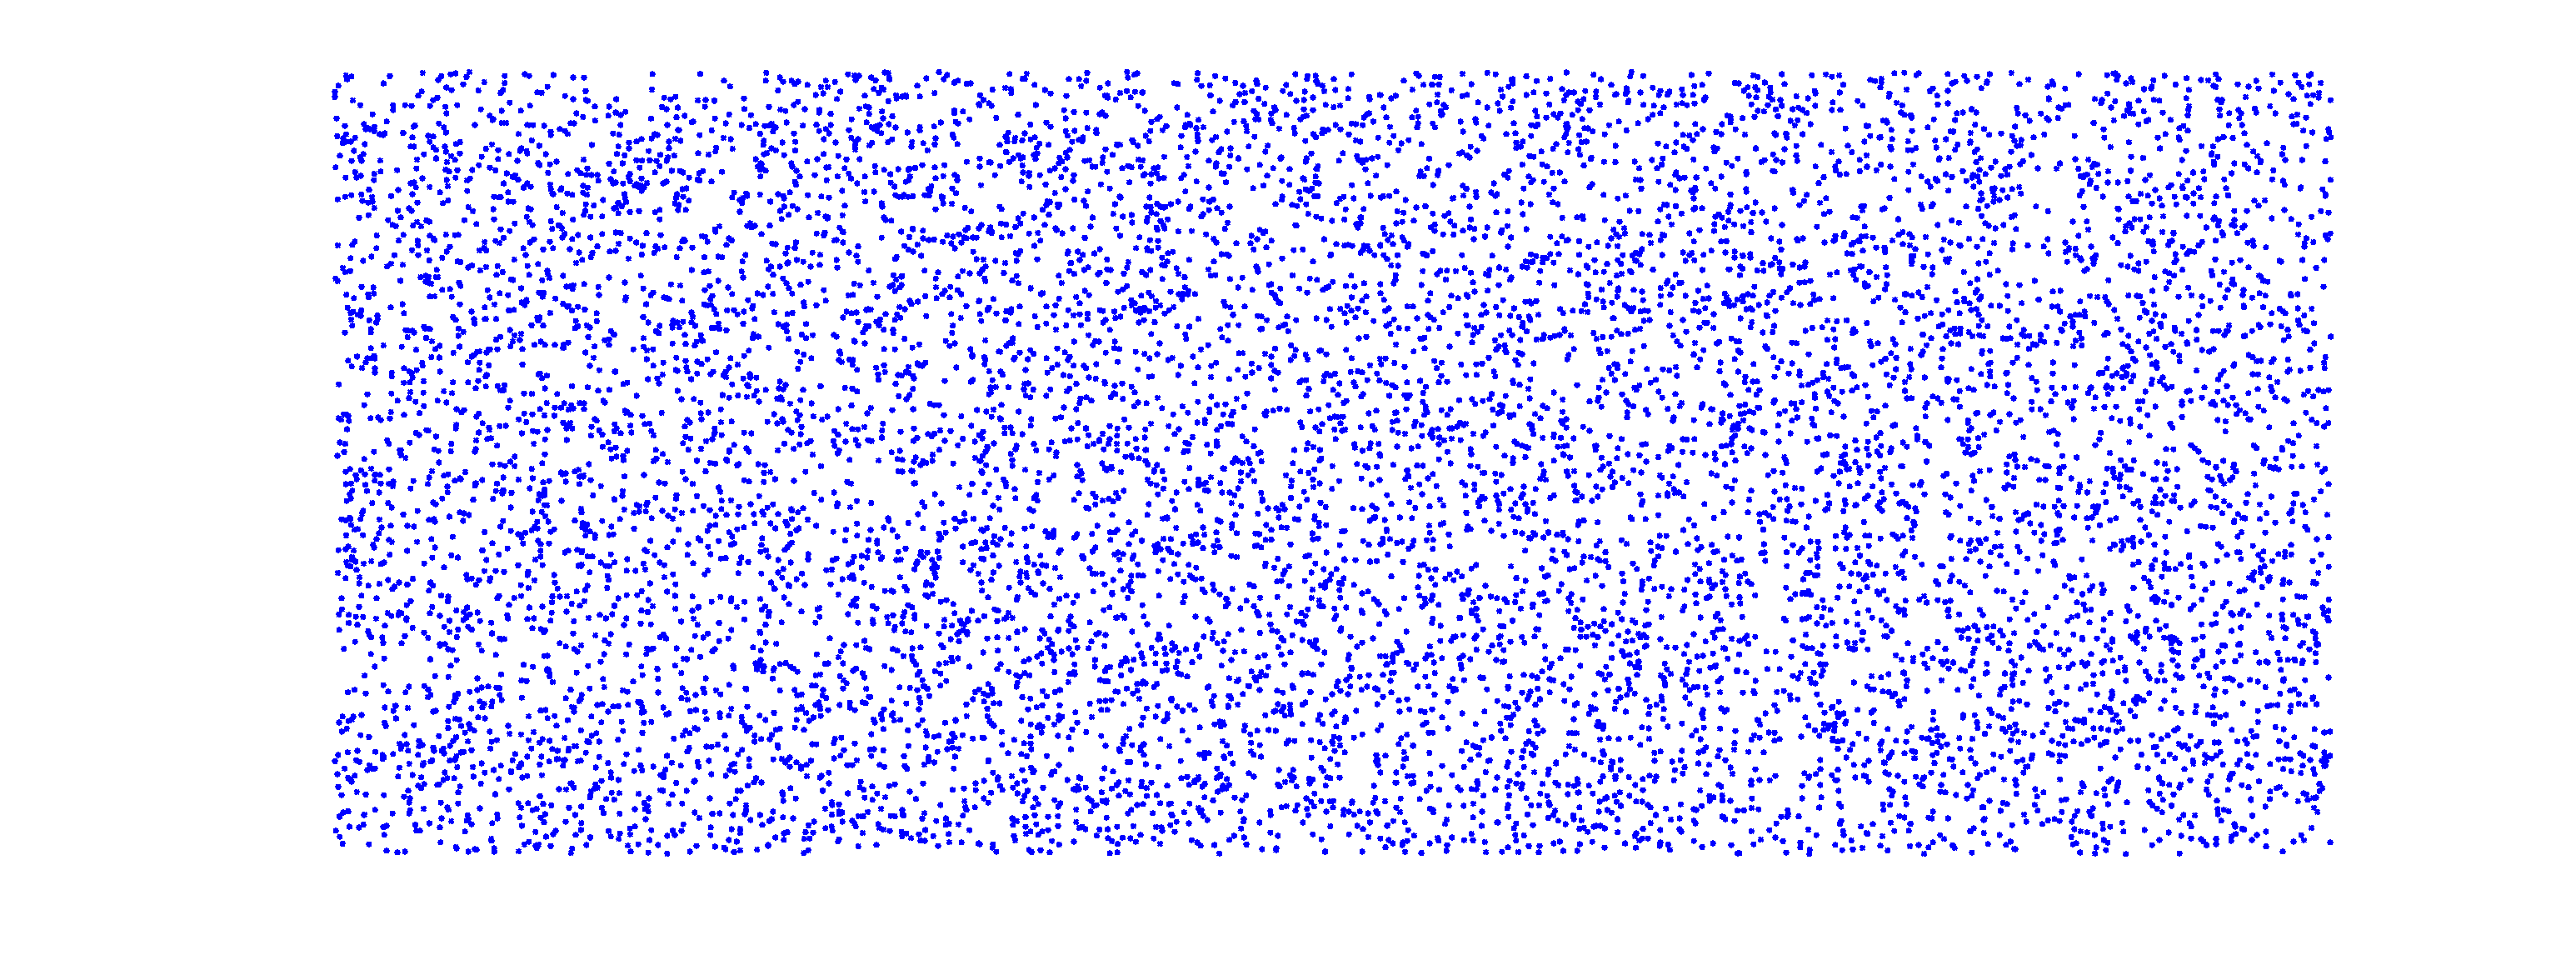
\includegraphics[height=10cm, width = 10cm]{figures/MCpoints}
\end{column}

\begin{column}{12cm}{\centering \scriptsize{Quasi-Monte Carlo (QMC)}}
\centering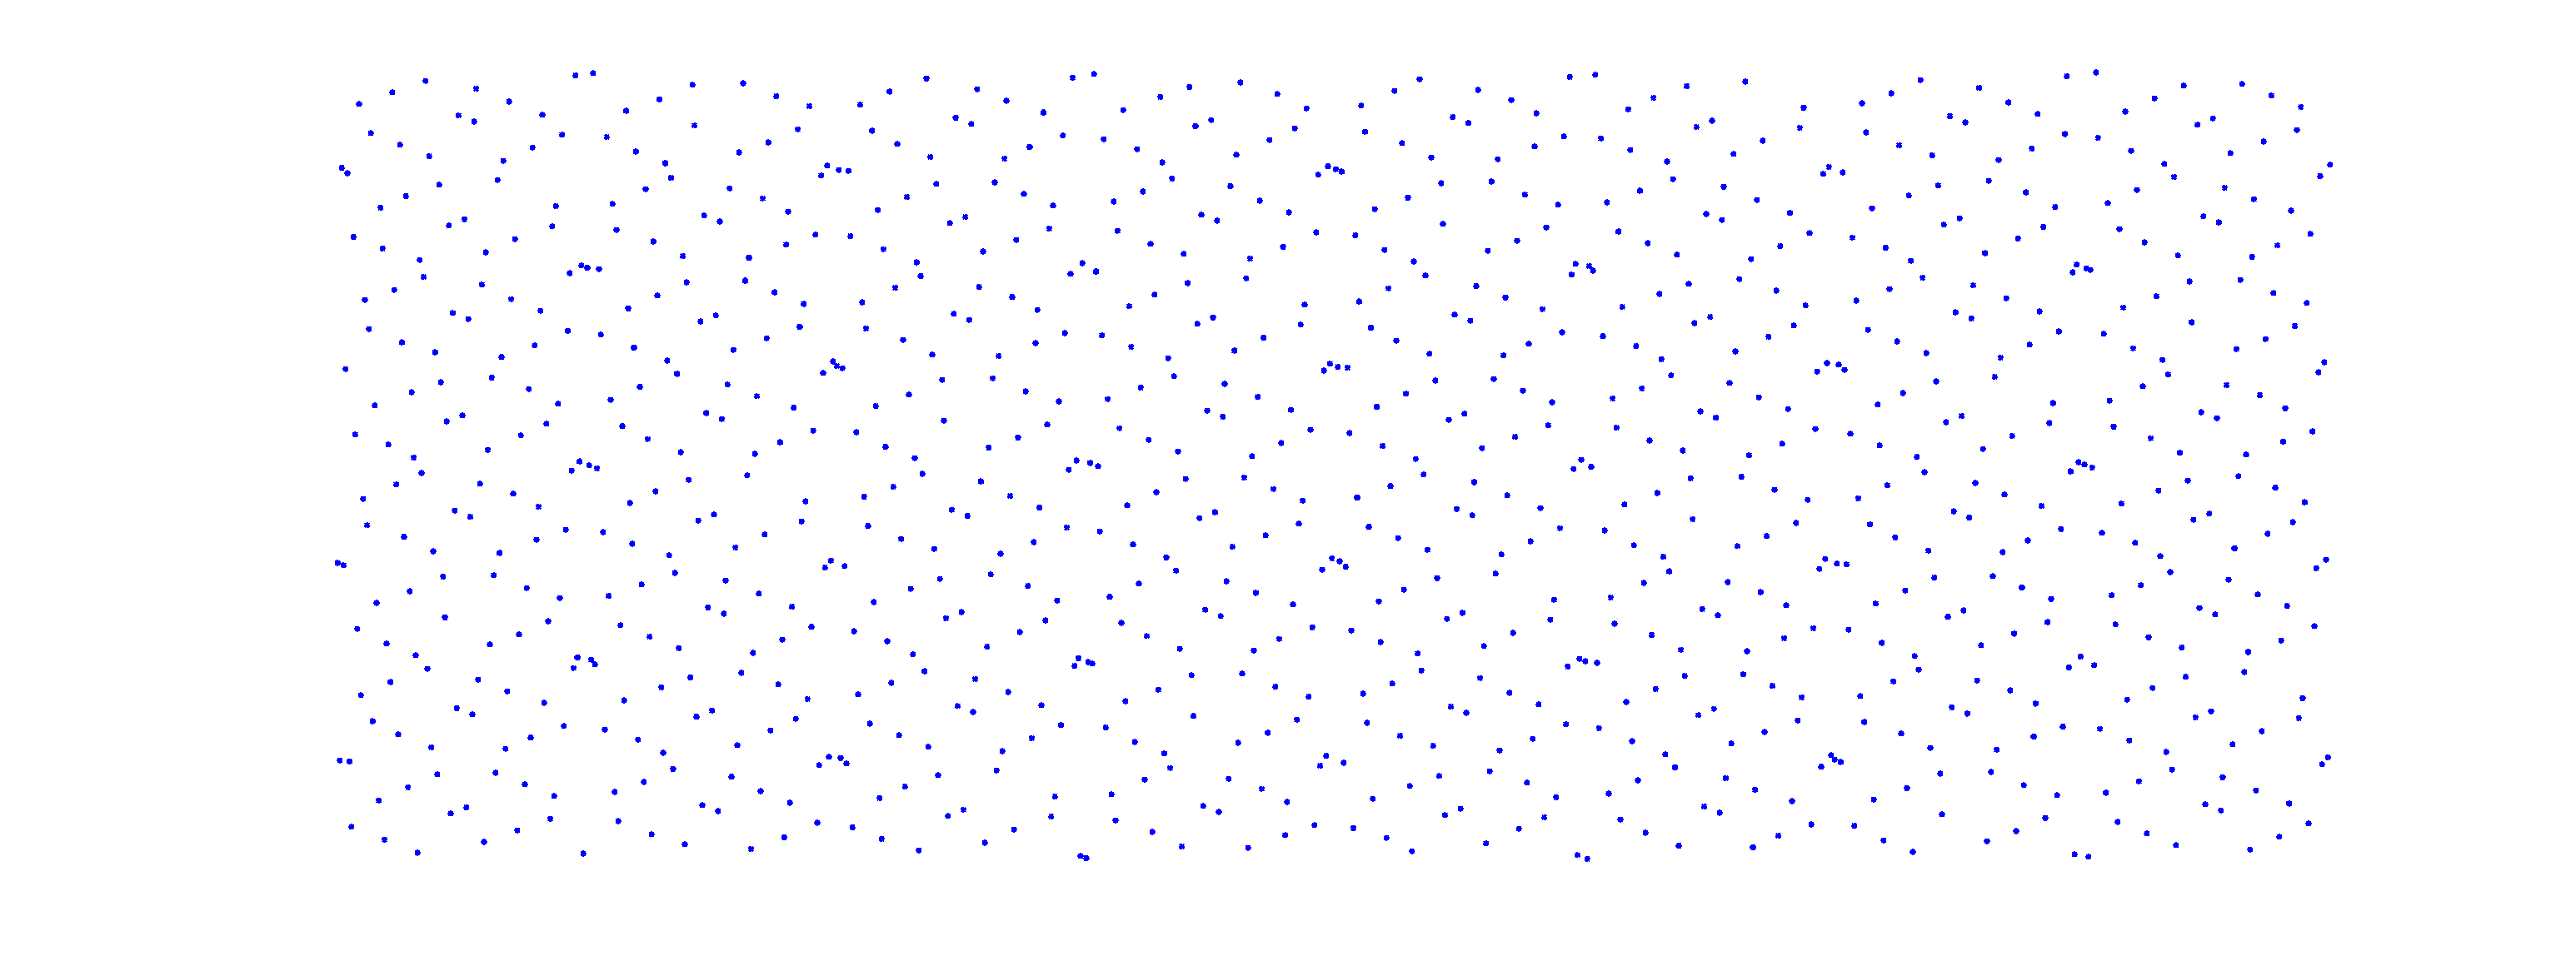
\includegraphics[height=10cm, width = 10cm]{figures/Sobolpoints}
\end{column}
\end{columns}

\vspace{0.5em}

\begin{columns}[T]

\begin{column}{10cm}{}
\centering
\vspace{3em}
$\E[f] = \sum\limits_{i=1}^M \omega_i f(\bxi_i)$
%$f\in \text{span}\{\prod\limits_{i=1}^d \xi_i^{p_i}\}$
\end{column}

\begin{column}{12cm}{\centering \scriptsize{Tensor Product (TP)}}
\centering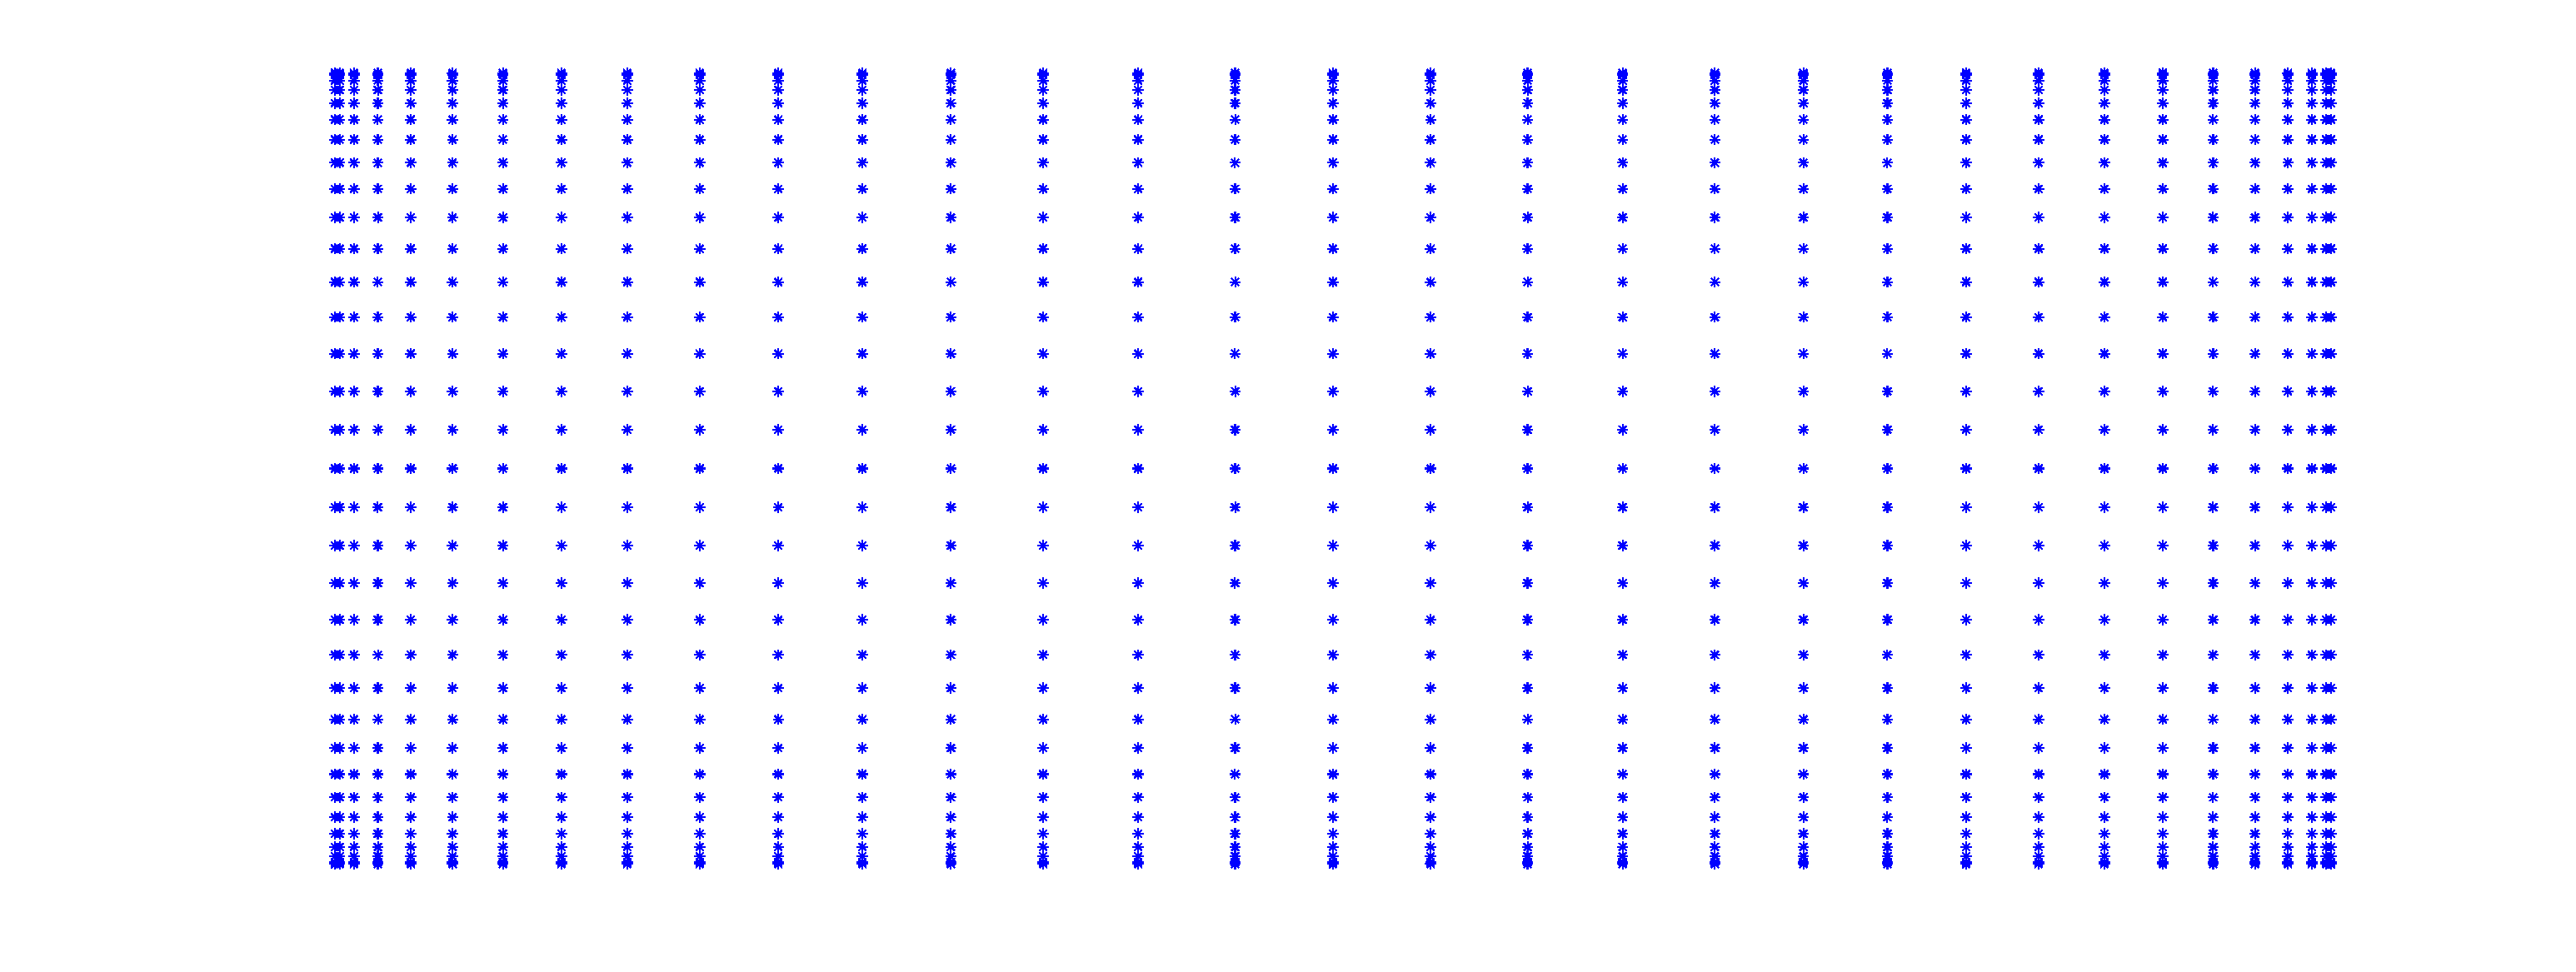
\includegraphics[height=10cm, width = 10cm]{figures/tensorproductpoints}
\end{column}

\begin{column}{12cm}{\centering \scriptsize{Sparse Grid (SG)}}
\centering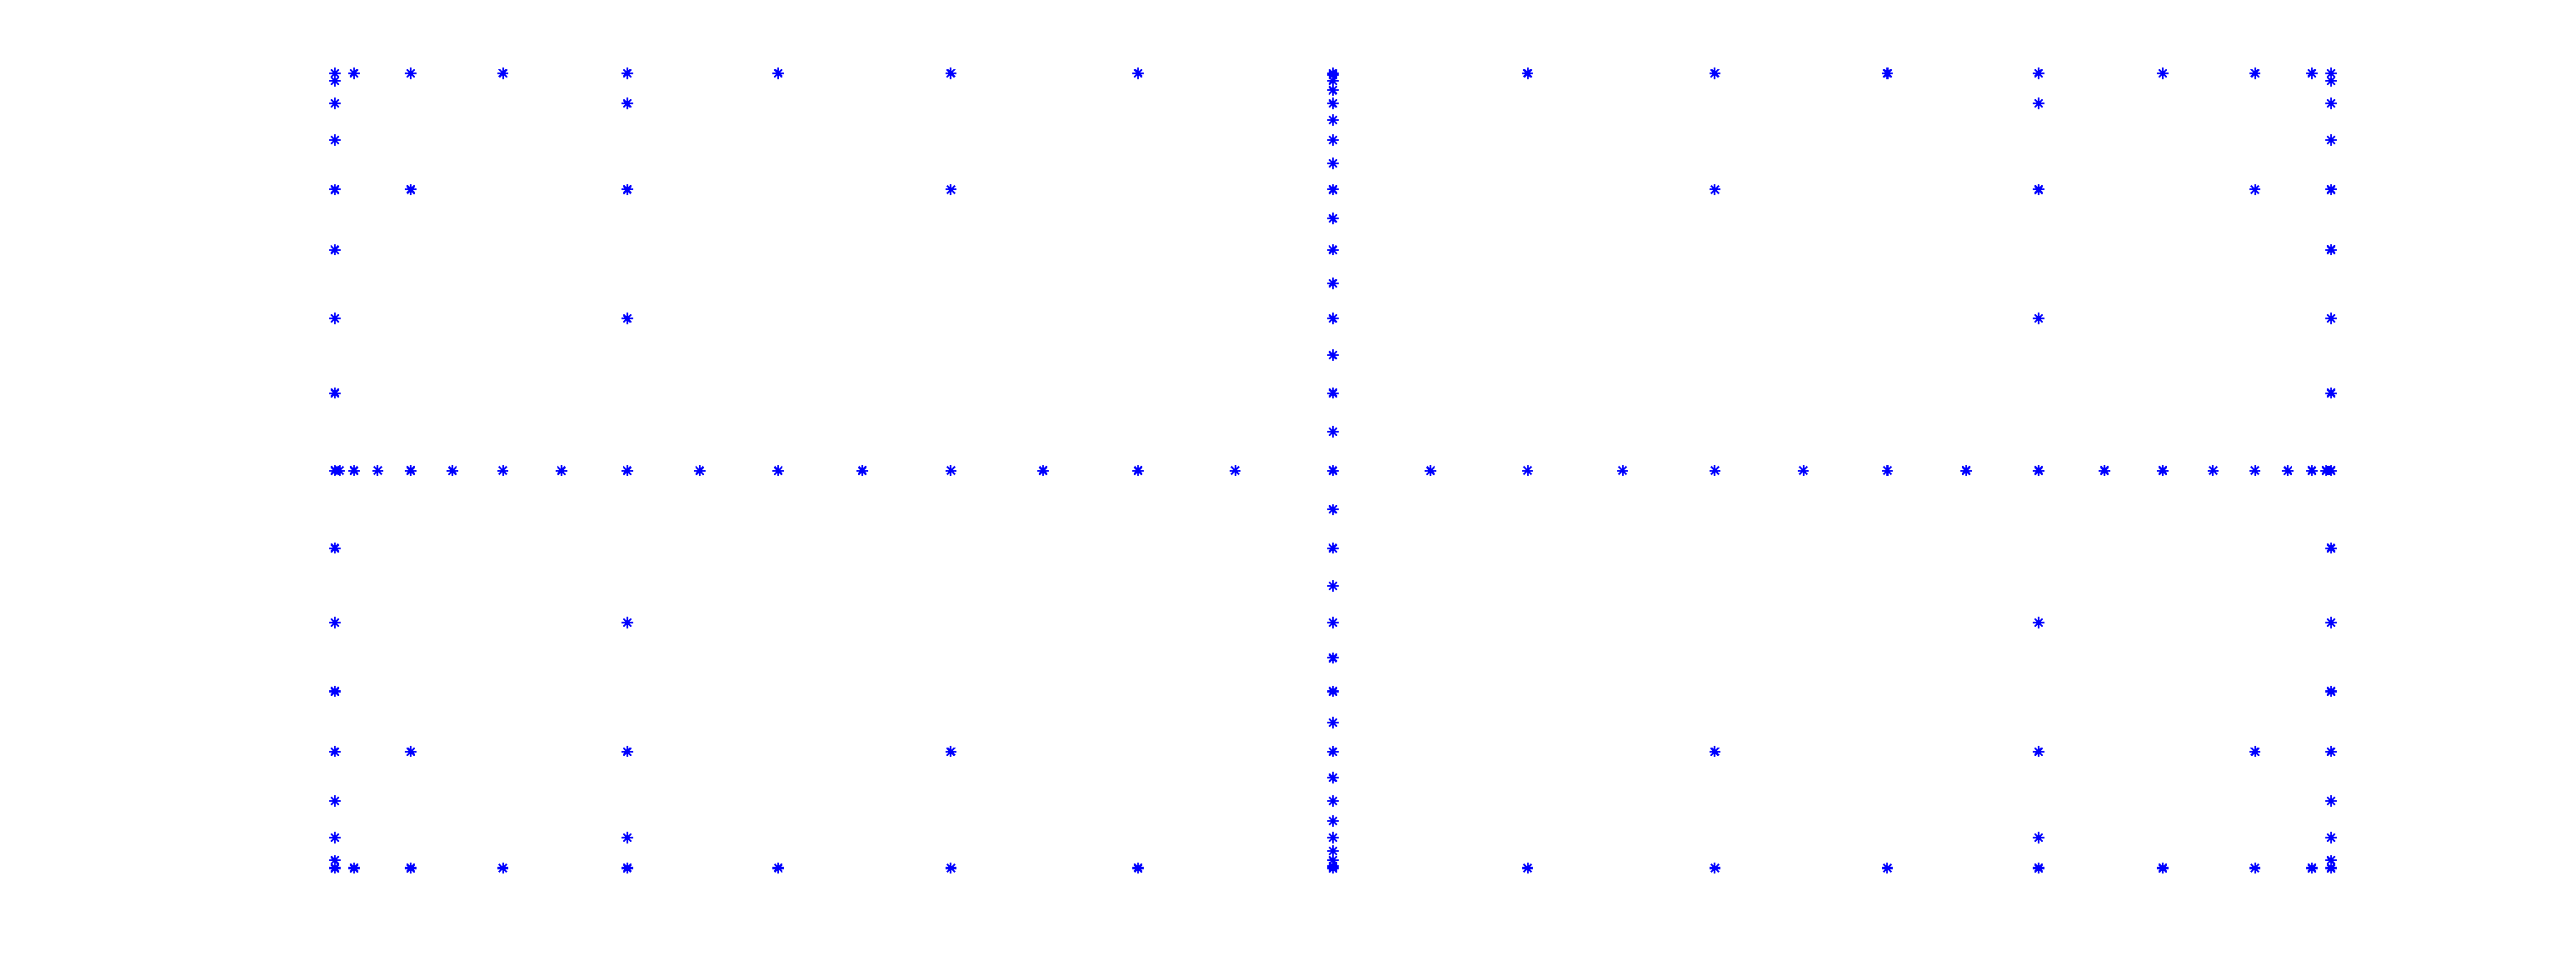
\includegraphics[height=10cm, width = 10cm]{figures/smolyakpoints}
\end{column}
\end{columns}


\end{block}
                
\begin{block}{\centering Optimizing the Optimizer}

\vspace{1em}

\begin{columns}[T]
\begin{column}{22cm}{}
Represent $f$ using hierarchical basis functions (with varying support):\\
\begin{equation*}
f(\bxi) \approx \sum\limits_{\bl} f_{\bl}(\bxi), \;\;\; f_{\bl}(\bxi) = \sum\limits_{\bi\;\;\text{odd}}  s_{\bl,\bi} \phi_{\bl,\bi}(\bxi)
\end{equation*}
%\noindent
%where coefficients $s_{\bl,\bi}$ are determined from 
%\begin{equation*}
%s_{\bl,\bi} = ( \prod_{j=1}^d [\; -\frac{1}{2} \;\; 1 \;\; -\frac{1}{2} \;]_{\xi_{l_j,i_j},l_j} ) f
%\end{equation*}
\noindent
where $d$-dimensional functions $\phi_{\bl,\bi}(\bxi)$ are defined as
\begin{equation*}
\phi_{\bl,\bi}(\bxi) = \prod_{j=1}^d \phi_{l_j,i_j}(\xi_j)
\end{equation*}
Coefficients $s_{\bl,\bi}$ are called \textit{hierarchical surpluses} as they represent hierarchichal increments between neighboring levels.
\end{column}
\begin{column}{12cm}{}
\centering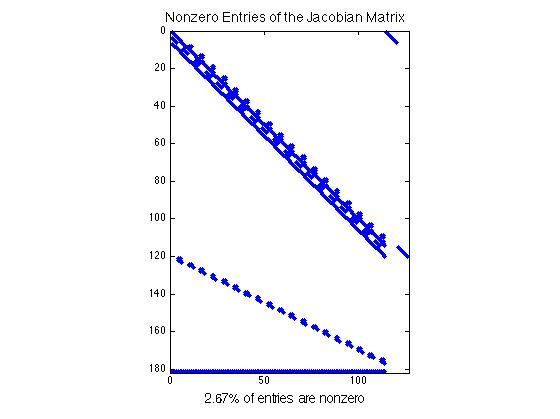
\includegraphics[height=16cm, width = 10cm]{figures/Spy_Jacobian.jpg} \\
\vspace{1em}
\centering \scriptsize{1D hierarchical piecewise linear basis}
\end{column}
%\begin{column}{16cm}{}
%\includegraphics[height=12cm, width = 14cm]{figures/hiersubspaces} \\
%Scheme of hierarchical subspaces in 2D
%\end{column}
\end{columns}


\end{block}
%-*-*-*-*-*-*-*-*-*-*-*-*-*-*-*-*-*-*-*-*-*-*-*-*untitled.eps-*-*-*-*-*-*-*-*-*-*-*-*-*-*-*-*-*-*-*-*               
%  \vspace{1cm}
                
 \begin{block}{\centering Optimality}

Hierarchical surpluses $s_{\bl,\bi}$ are a natural local error indicator.\\

Thus, refining only points with relatively large surpluses we obtain an adaptive grid (with more points spent in non-smooth areas).\\
%
%The idea of adaptivity is to refine only those points $\bxi_{\bl,\bi}$ for which $|s_{\bl,\bi}|>\epsilon$ (where $\epsilon$ is prescribed tolerance).\\

%1D example\\
\begin{columns}[T]
\begin{column}{16cm}{}
\centering 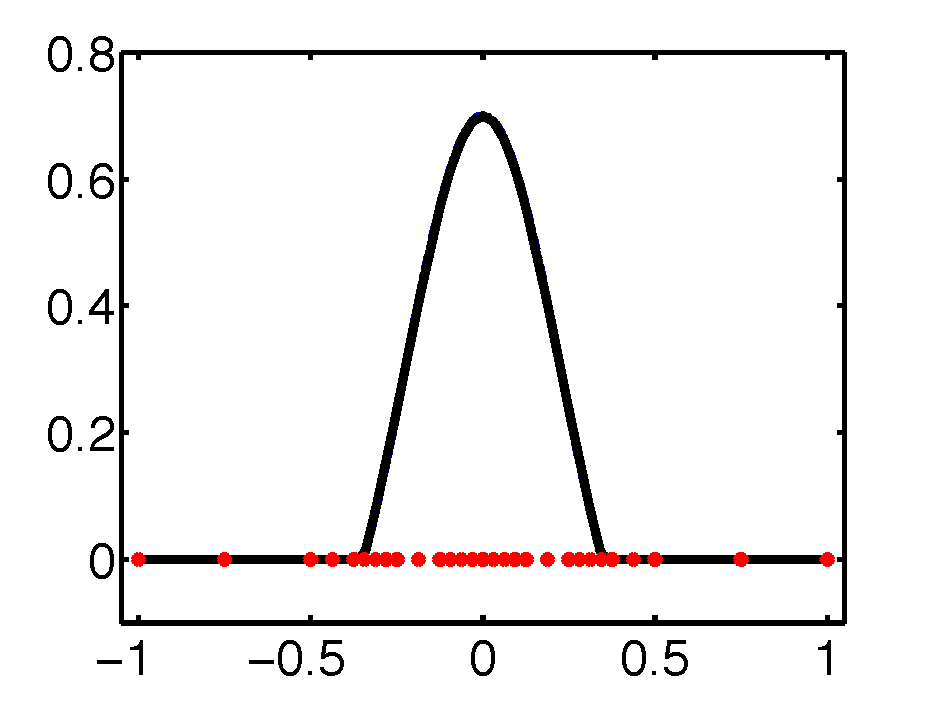
\includegraphics[height=10cm, width = 16cm]{figures/1Dadaptivefunc}\\
\centering \scriptsize{Adaptive grid}
%$f(\xi) = \max{\{\exp{(-10\xi^2)}-0.3,0\}}$
\end{column}
\begin{column}{16cm}{}
\raggedleft 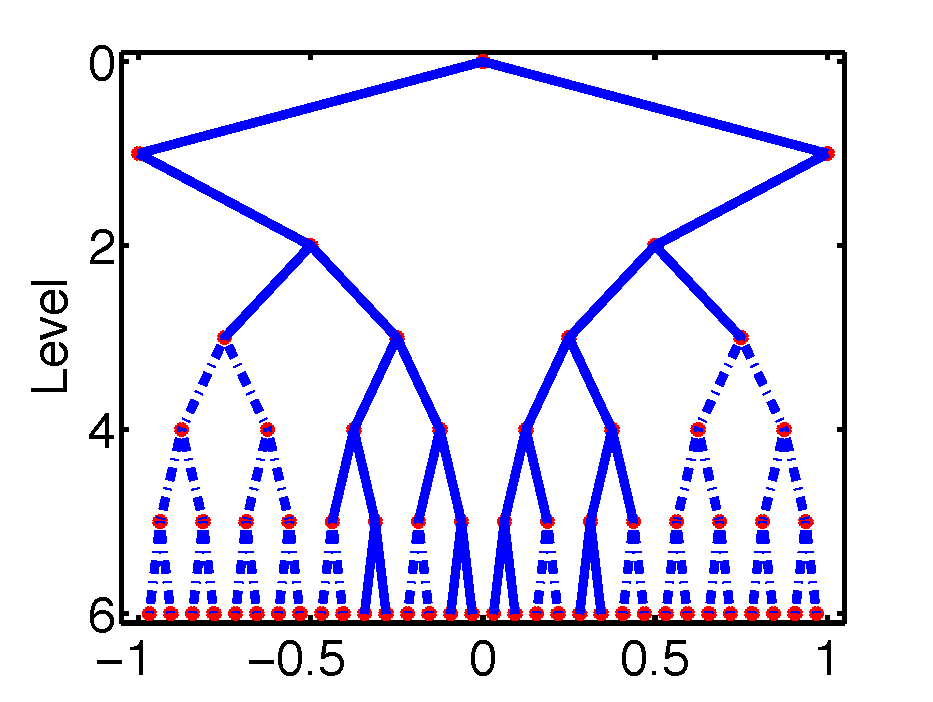
\includegraphics[height=10cm, width = 16cm]{figures/1Dadaptivetree}\\
\centering \scriptsize{Adaptivity tree}
\end{column}
\end{columns}

%\vspace{1cm}
%
%Application to function $f_2(\bxi)$
%\begin{columns}[T]
%\begin{column}{16cm}{}
%\includegraphics[height=10cm, width = 10cm]{figures/hierpoly1points}\\
%Adaptive sparse grid
%\end{column}
%\begin{column}{16cm}{}
%\includegraphics[height=10cm, width = 14cm]{figures/errornonsmoothH}\\
%Error in integral
%\end{column}
%\end{columns}

\end{block}

 \end{column}
% =============================================================================
%                                     Column 3
% =============================================================================
        
\begin{column}{.30\linewidth}

\begin{block}{\centering Dog Pics} 
\vspace{-1em}
\begin{columns}[T]
\begin{column}{18cm}{}
\centering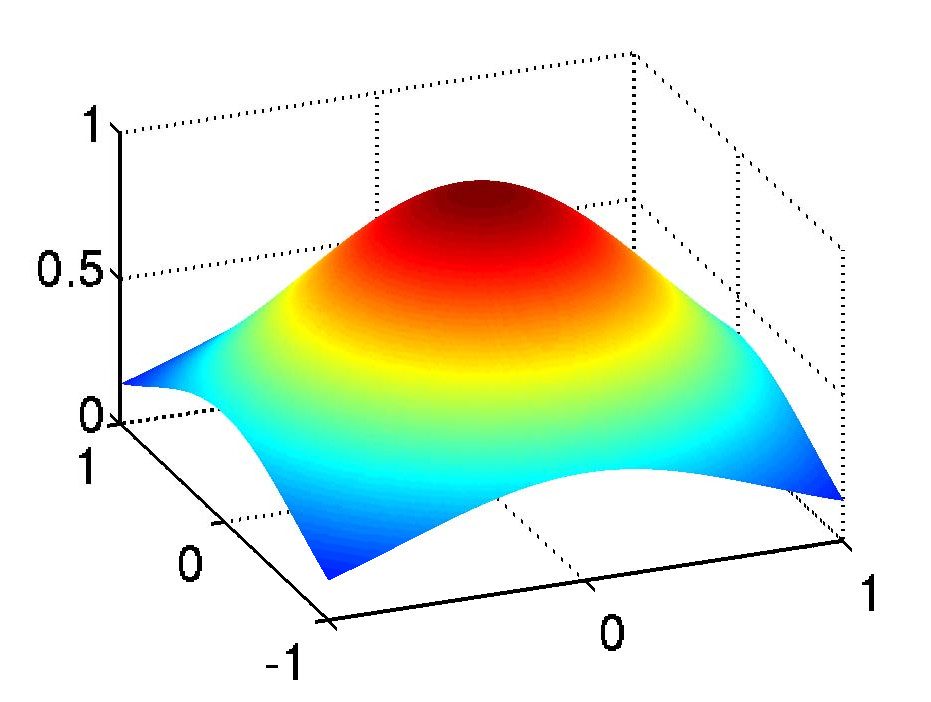
\includegraphics[height=10cm, width = 14cm]{figures/gaussian}\\
\centering\scriptsize{$f_1(\bxi) = \exp{(-\sum\limits_{i=1}^d \xi_i^2)}$}
%Smooth with respect to parameters
\end{column}
\begin{column}{18cm}{}
\centering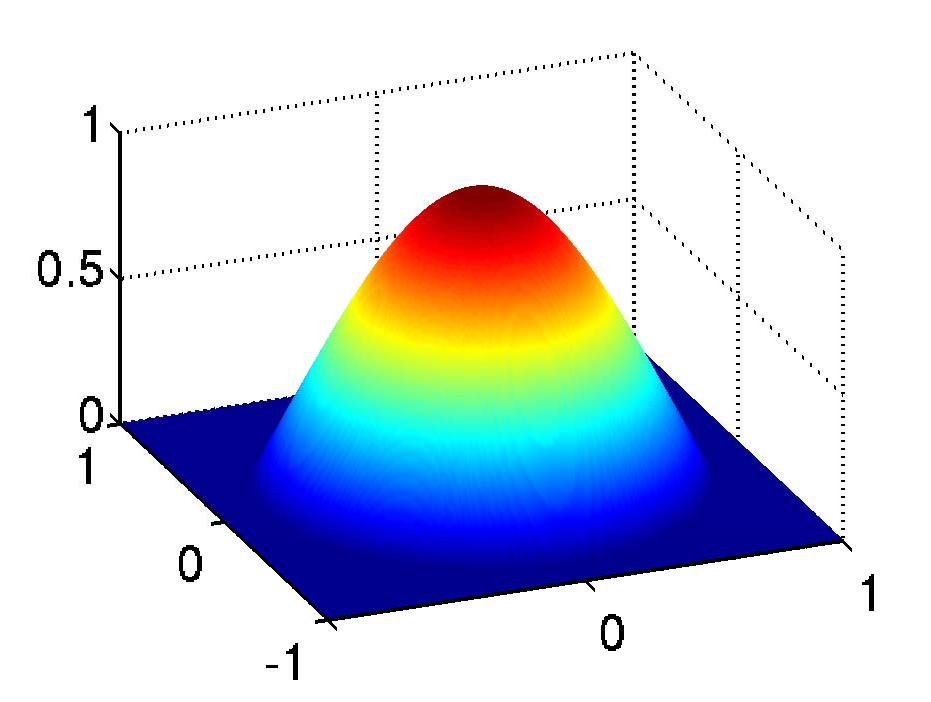
\includegraphics[height=10cm, width = 14cm]{figures/maxgaussian}\\
\centering\scriptsize{$f_2(\bxi) = 2\max{\{f_1(\bxi)-\frac{1}{2},0\}}$}
%Non-smoothness introduced by max function
\end{column}
\end{columns}

\vspace{0.5em}
\begin{columns}[T]

\begin{column}{12cm}{}
\centering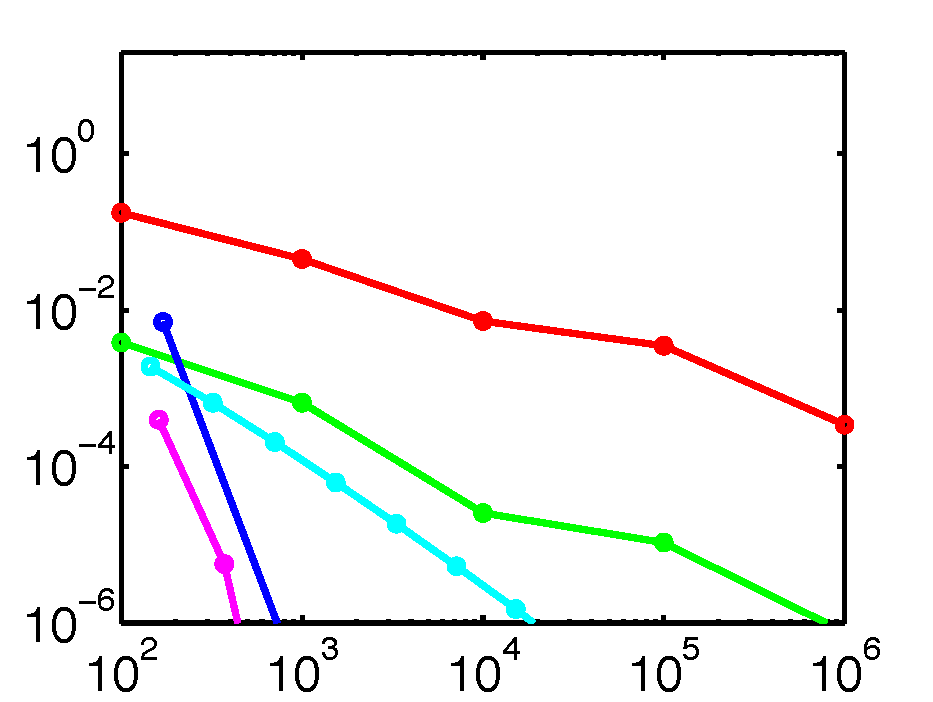
\includegraphics[height=10cm, width = 14cm]{figures/gaussian2errors}\\

\end{column}
\begin{column}{4cm}{}
\vspace{2cm}
\centering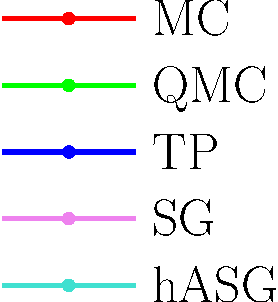
\includegraphics[height=5cm,width=5cm]{figures/legend}\\
\end{column}
\begin{column}{14cm}{}
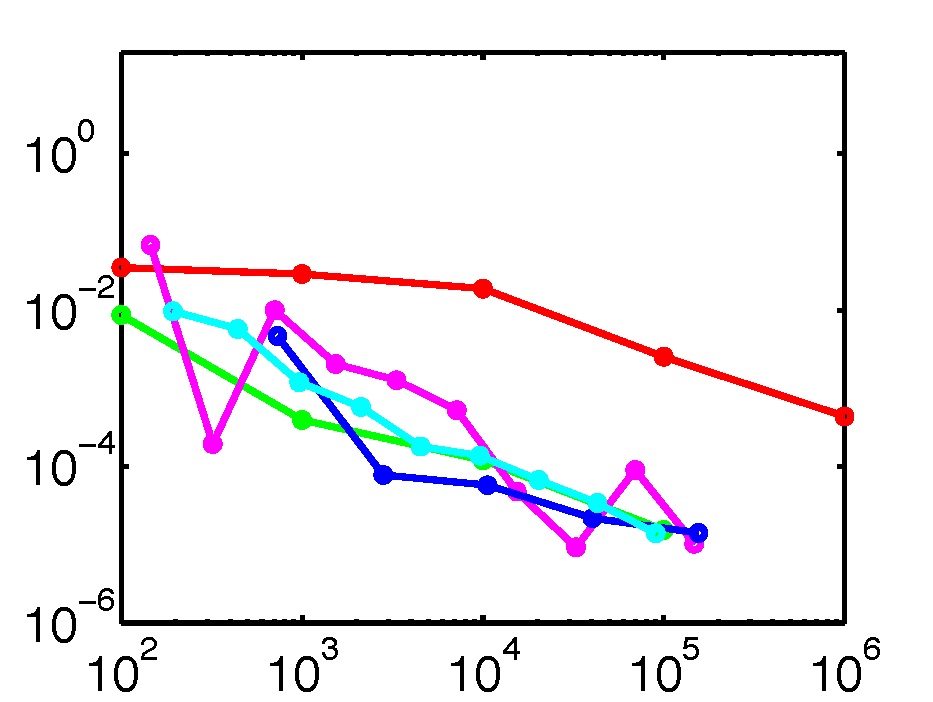
\includegraphics[height=10cm, width = 14cm]{figures/maxgaussian2errors}\\
%Deterioration in rates of convergence for $f_2(\xi_1,\xi_2)$
\end{column}
\end{columns}
\vspace{0.5em}
\centering\scriptsize{Absolute errors in integral vs the number of samples for $d=2$}

\begin{columns}[T]
\begin{column}{12cm}{}
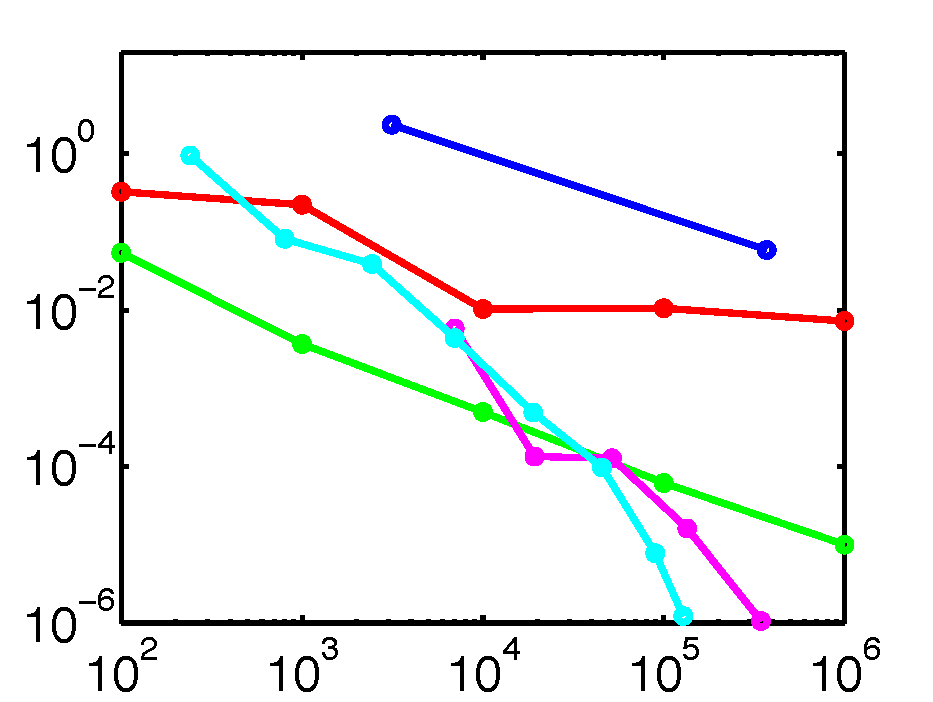
\includegraphics[height=10cm, width = 14cm]{figures/gaussian5errors}\\
%Rates of convergence for $f_1(\xi_1,\xi_2)$
\end{column}
\begin{column}{4cm}{}
\vspace{2cm}
\centering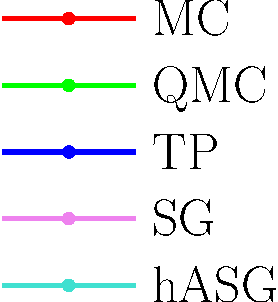
\includegraphics[height=5cm,width=5cm]{figures/legend}\\
\end{column}
\begin{column}{14cm}{}
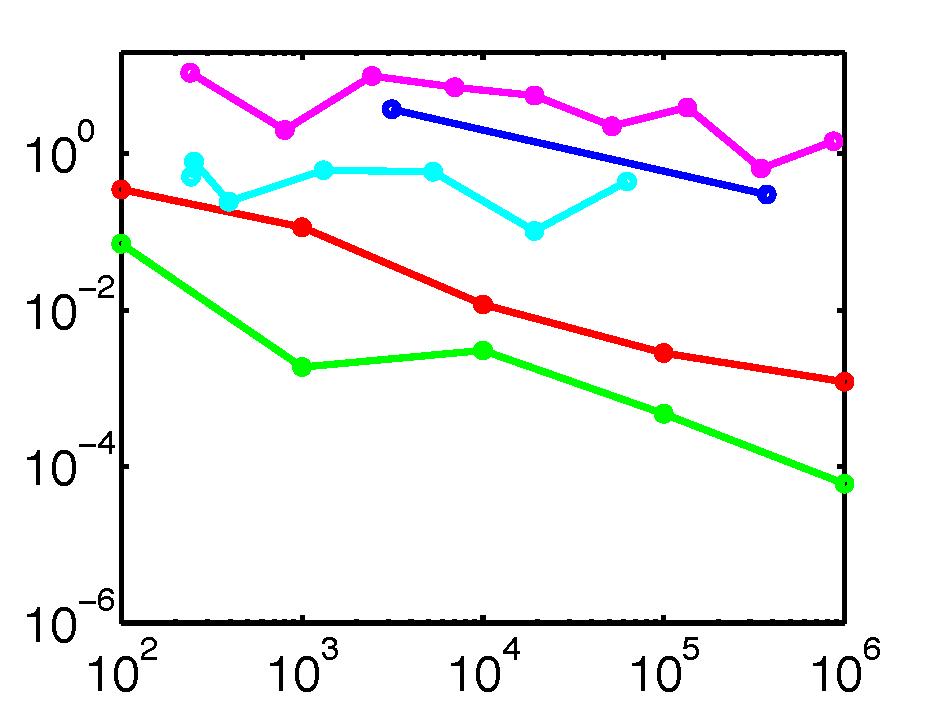
\includegraphics[height=10cm, width = 14cm]{figures/maxgaussian5errors}\\
%Deterioration in rates of convergence for $f_2(\xi_1,\xi_2)$
\end{column}
\end{columns}
\vspace{0.5em}
\centering\scriptsize{Absolute errors in integral vs the number of samples for $d=5$}

\end{block}

                
\begin{block}{\centering Results}
\vspace{-0.5em}
\begin{columns}[T]
\begin{column}{12cm}{}
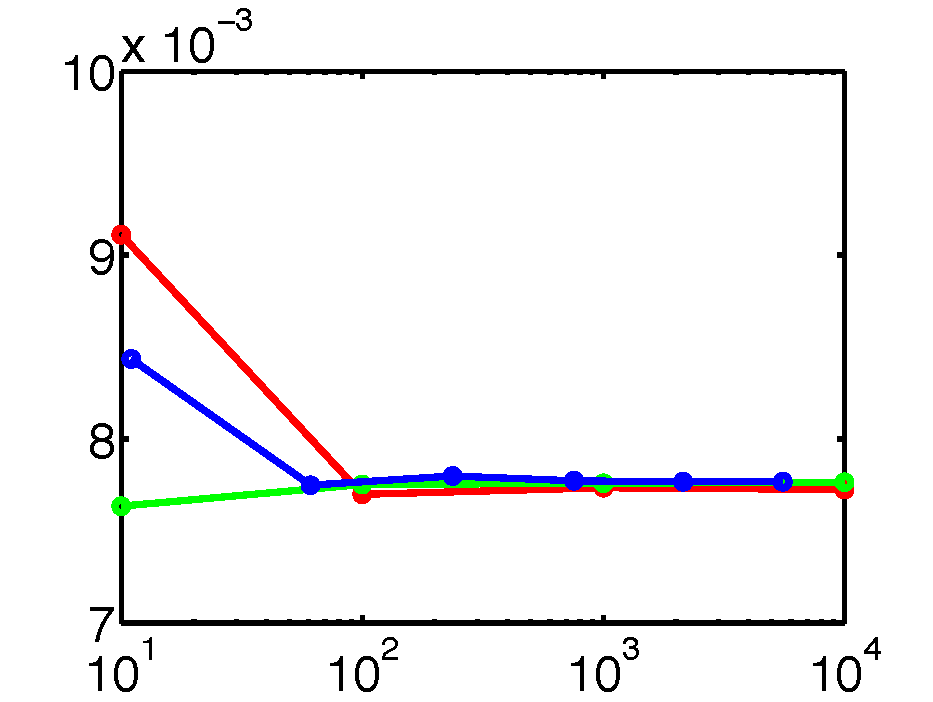
\includegraphics[height=10cm, width = 14cm]{figures/exp5errors}\\
%Rates of convergence for exp
\end{column}
\begin{column}{4cm}{}
\vspace{2cm}
\centering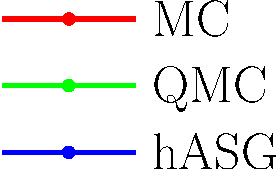
\includegraphics[height=3cm,width=5cm]{figures/legend2}\\
\vspace{1em}
\centering{\footnotesize{$N=5$}}
\end{column}
\begin{column}{14cm}{}
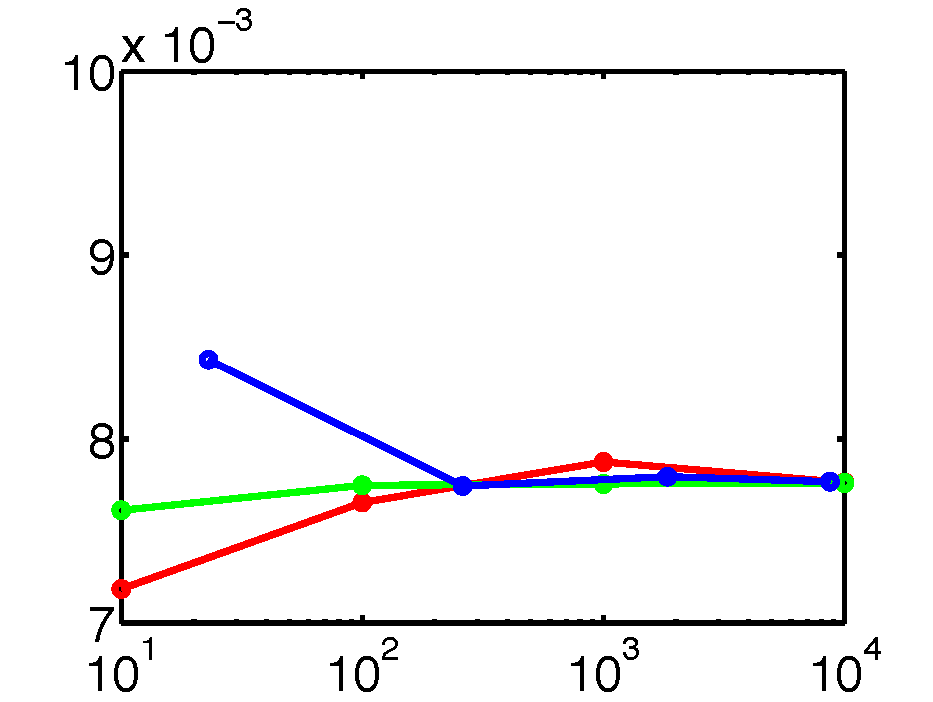
\includegraphics[height=10cm, width = 14cm]{figures/exp11errors}\\
%Deterioration in rates of convergence for exp
\end{column}
\end{columns}
\vspace{0.5em}
\centering\scriptsize{Approximation of the mean value vs the number of samples}
%: $\E[Q(u(\cdot,\bx))]$
\vspace{-0.5em}
\begin{columns}[T]
\begin{column}{12cm}{}
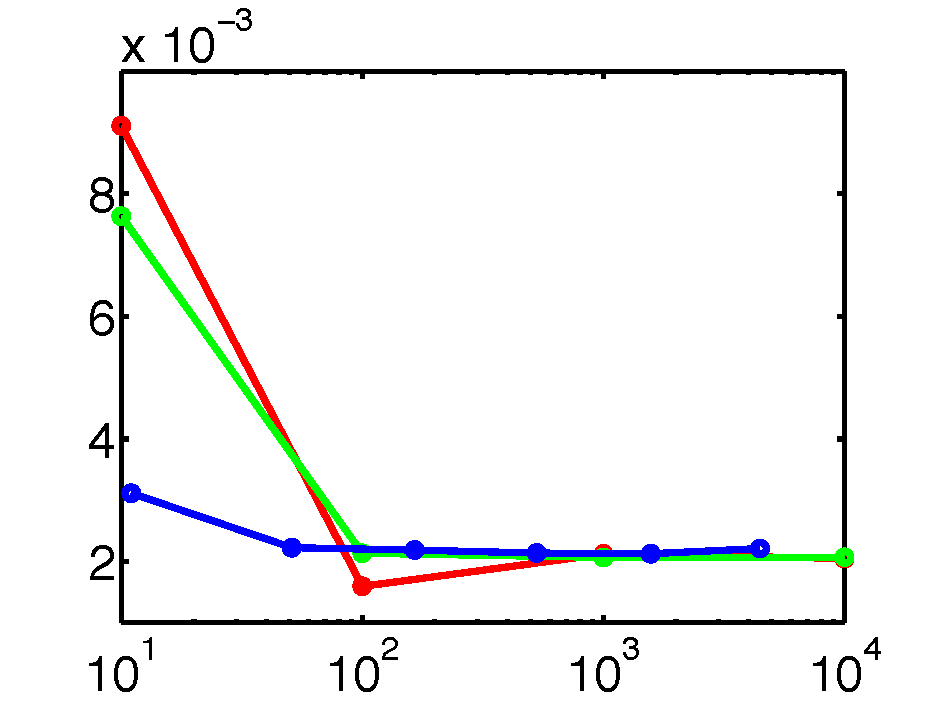
\includegraphics[height=10cm, width = 14cm]{figures/semidev5errors}\\
%Rates of convergence for semidev
\end{column}
\begin{column}{4cm}{}
\vspace{2cm}
\centering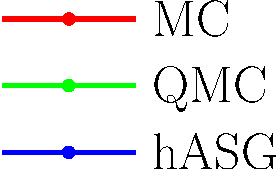
\includegraphics[height=3cm,width=5cm]{figures/legend2}\\
\vspace{1em}
\raggedright{\footnotesize{$N=11$}}
\end{column}
\begin{column}{14cm}{}
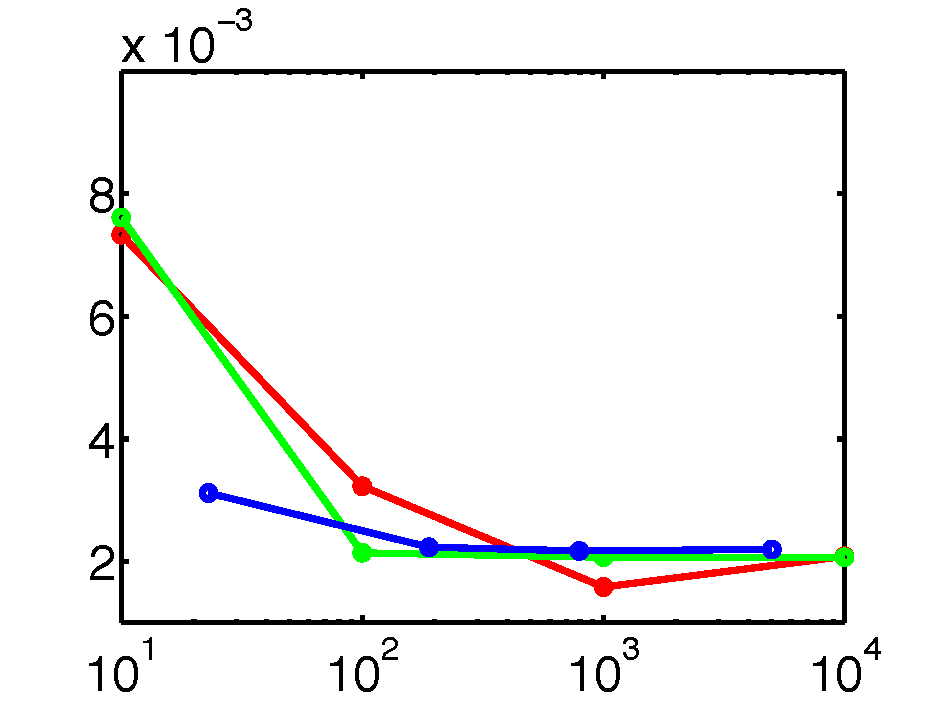
\includegraphics[height=10cm, width = 14cm]{figures/semidev11errors}\\
%Deterioration in rates of convergence for semidev
\end{column}
\end{columns}
\vspace{0.5em}
\centering\scriptsize{Approximation of the semi-deviation vs the number of samples}
%: $\E[\max{\{(Q(u(\cdot,\bx)) - \E[Q(u(\cdot,\bx))]),0\}}]$
\end{block}



                
%-*-*-*-*-*-*-*-*-*-*-*-*-*-*-*-*-*-*-*-*-*-*-*-*-*-*-*-*-*-*-*-*-*-*-*-*-*-*-*-*-*-*-*-*             
%  \vspace{1cm}
                
\begin{block}{\centering Future work}
\begin{itemize}
	\item Finding the reason for occasional failure of optimizing with MATLAB's fmincon
	\item Investigating why the minimum time path is asymmetric from belt to goal and vice versa
\end{itemize}
\end{block}
                
%-*-*-*-*-*-*-*-*-*-*-*-*-*-*-*-*-*-*-*-*-*-*-*-*-*-*-*-*-*-*-*-*-*-*-*-*-*-*-*-*-*-*-*-*                
% \vspace{0.5cm}
                
%                \setbeamertemplate{
%bibliography item}[text] % for numbering on the references

%               \begin{block}{References}
%                       \bibliographystyle{plain}
%                       \begin{thebibliography}{99}
                
                        %{\scriptsize \bibliography{refs}}
%\tiny \bibitem{SS} [1] F. Santosa and W. Symes, \textit{Linear Inversion of Band-Limited Reflection Seismograms,} 1986
%\tiny \bibitem{GRB} [2] Gurobi Optimization, \textit{Gurobi Optimizer Reference Manual,} 2012, \\ \url{www.gurobi.com}.
%\tiny \bibitem{RECPF} [3] J. Yang, Y. Zhang and W. Yin, \textit{A Fast Alternating Direction Method for TVL1-L2 signal reconstruction from Partial Fourier Data,} April 2010, \\
%\url{www.caam.rice.edu/~optimization/L1/RecPF/}.

                    
   %                 \end{thebibliography}
                       
                    
        %               \vspace{.05cm}
                %\end{block}
                
                %-*-*-*-*-*-*-*-*-*-*-*-*-*-*-*-*-*-*-*-*-*-*-*-*-*-*-*-*-*-*-*-*-*-*-*-*-*-*-*-*-*-*-*-*
                
%                \vspace{1cm}
                
%                \begin{block}{Aknowledgements}
%                
%                This work is partially funded by NSF Grant DMS-0811188 and DMS-1115950 and by CONACYT.
%                        %{\scriptsize
%        
%                                %\begin{figure}
%                                %\includegraphics{rice-logo} \hspace{1cm} 
%                                %\includegraphics{conacyt}\hspace{1cm} \includegraphics[width=2in]{nsf}
%                                %\end{figure}
%
%                                %  \center{ \tiny This work is partially funded by NSF Grant DMS-0811188 and DMS-1115950 and by CONACYT. }
%                        %}
%                \end{block}
                
\end{column}
        
\end{columns}
}       % end of footnotesize

\end{frame}
        
\end{document} %===================================================================================
%==================================================================================================
%%
%% \begin{block}{\large Fontsizes}
%%       \centering
%%       {\tiny tiny}\par
%%       {\scriptsize scriptsize}\par
%%       {\footnotesize footnotesize}\par
%%       {\normalsize normalsize}\par
%%       {\large large}\par
%%       {\Large Large}\par
%%       {\LARGE LARGE}\par
%%       {\veryHuge veryHuge}\par
%%       {\VeryHuge VeryHuge}\par
%%       {\VERYHuge VERYHuge}\par
%% \end{block}
%%
%%====================================================
%%
%%      \begin{block}{Methods}
%%              \begin{figure}[htbp]
%%                      \begin{center}
%%                              \includegraphics[width=7in]{lp_example2.pdf}
%%                              \label{ fig:lp_example1.pdf}
%%                      \end{center}
%%              \end{figure}
%%      \end{block}
%%
%%%%%%%%%%%%%%%%%%%%%%%%%%%%%%%%%%%%%%%%%%%%%%%%%%%%%%%%%%%%%%%%%%%%%%%%%%%%%%%%%%%%%%%%%%%%%%%%%%%%
%%% Local Variables: 
%%% mode: latex
%%% TeX-PDF-mode: t
